\documentclass[a4paper,11pt,fleqn]{article}%fleqn pour aligner les equations à gauche
\usepackage{../../Styles/Cours}

\newcommand{\chnum}{Chapitre 18}
\newcommand{\chtitle}{Conditions d'interférences}
\newcommand{\dtype}{Activité}
  
\begin{document}
\maketitle
Deux perturbations à la surface de l'eau produisent des ondes qui se propagent et se rencontrent. \textbf{Comment expliquer ce que l'on observe à la surface de l'eau quand les deux ondes se croisent ?}

\begin{figure}[h!]
  \begin{minipage}{.48\linewidth}
    \caption{Ondes à la surface de l'eau}
    \label{doc1}
    Les vibrations périodiques d'une poine $S$ à la surface de l'eau d'une cuve à onde (a) créent des ondes circulaires périodiques se propageant de façon concentriques à la surface de l'eau. l'alternance de ces crètes (traits pleins) et des creux (pointillés) de l'onde est représentée ci-dessous (b). l'état vibratoire d'un point de la surface est appélé \emph{phase}.
    \begin{center}
      
    \begin{tikzpicture}
      %\draw (0,0) rectangle(8,2);
      \fill[top color =blue!30] (0,0) -- plot[smooth,domain = 0:5,samples=200](\x, {.25*sin(300*\x-40)+1})
      -- plot[smooth,domain = 5:8,samples=200](\x, {.25*sin(300*\x+100)+1})
      --(8,0) --cycle;

      \draw[blue,very thick] plot[smooth,domain = 0:5,samples=200](\x, {.25*sin(300*\x-40)+1});

      \draw[blue,very thick] plot[smooth,domain = 5:8,samples=200](\x, {.25*sin(300*\x+100)+1});

      %\draw(0,0) grid(8,2);
      %\draw (0,-3) rectangle(8,0);
      
      \shade[outer color= blue!20, inner color = white] (2.85,-3) arc(180:0:2.15)--cycle;
      \draw (2.85,-3) arc(180:0:2.15);
      \draw (2.85,-3) --(2.85,1.5);
      \draw (7.15,-3) --(7.15,1.5);
      
      
      \shade[outer color= blue!20, inner color = white] (3.45,-3) arc(180:0:1.55)--cycle;
      \draw[dashed] (3.45,-3) arc(180:0:1.55);
      \draw[dashed] (3.45,-3) --(3.45,.75);
      \draw[dashed] (6.55,-3) --(6.55,.75);
      
      
      \shade[outer color= blue!20, inner color = white] (4.05,-3) arc(180:0:.95)--cycle;
      \draw (4.05,-3) arc(180:0:.95);
      \draw (4.05,-3) --(4.05,1.5);
      \draw (5.95,-3) --(5.95,1.5);


      \shade[outer color= blue!20, inner color = white] (4.65,-3) arc(180:0:.35)--cycle;
      \draw[dashed] (4.65,-3) arc(180:0:.35);
      \draw[dashed] (4.65,-3) --(4.65,.75);
      \draw[dashed] (5.35,-3) --(5.35,.75);
      
      %%  Légendes

      \draw (1,1.25) node[above]{\textbf{a}};
      \draw (1,-.2) node{\textbf{b}};

      \draw (5,1.75) node[above]{\textbf{Pointe S}};
      \draw[-Stealth] (5,1.75) to (5,1.2);

      \draw[Stealth-Stealth] (5.35,.65) to (6.55,.65);
      \draw[Stealth-Stealth] (5.95,1.35) to (7.15,1.35);

      \draw (5.7,.65) node[below]{$\lambda$};
      \draw (6.55,1.35) node[above]{$\lambda$};

      \draw (5,-3) node[below]{\textbf{S}};

      \draw (1.75,-1) node{Crète};
      \draw (0.25,-1)--(1,-1);
      \draw (1.75,-2) node{Creux};
      \draw[dashed] (0.25,-2)--(1,-2);
      \draw (0,-2.5) rectangle(2.5,-.5);
    \end{tikzpicture}
    \end{center}
  \end{minipage}\hspace{.02\linewidth}
  \begin{minipage}{.5\linewidth}
    \caption{interférences entre deux ondes cohérentes}
    \label{doc2}
    Deux sources d'ondes vibrant à la même fréquence et avec un déphasage constant sont dites cohérentes. Les ondes produites par deux sources cohérentes se rencontrent et se superposent. L'état d'un point donné dépend de l'état vibratoire de chaque onde en ce point :
    \begin{itemize}
      \item les ondes sont en opposition de phase, les interférences dont destructives
      \item les ondes ne sont pas en opposition de phase, les interférences sont constructives avec une stituation extrême correspondant au cas où les deux ondes sont à leur extremum d'amplitude
    \end{itemize}
  \end{minipage}
\end{figure}
\begin{figure}
  \caption{Schémma de la situation}
  \label{doc3}
  L'interférence de deux ondes cohérentes est schématisée ci-après.\\
    $d_1$ et $d_2$ dont les distances entre un point de la surface et respectivement les sources 1 et 2. La différence entre ces deux distances est appelée différence de chemin $\delta$.
\begin{center}
  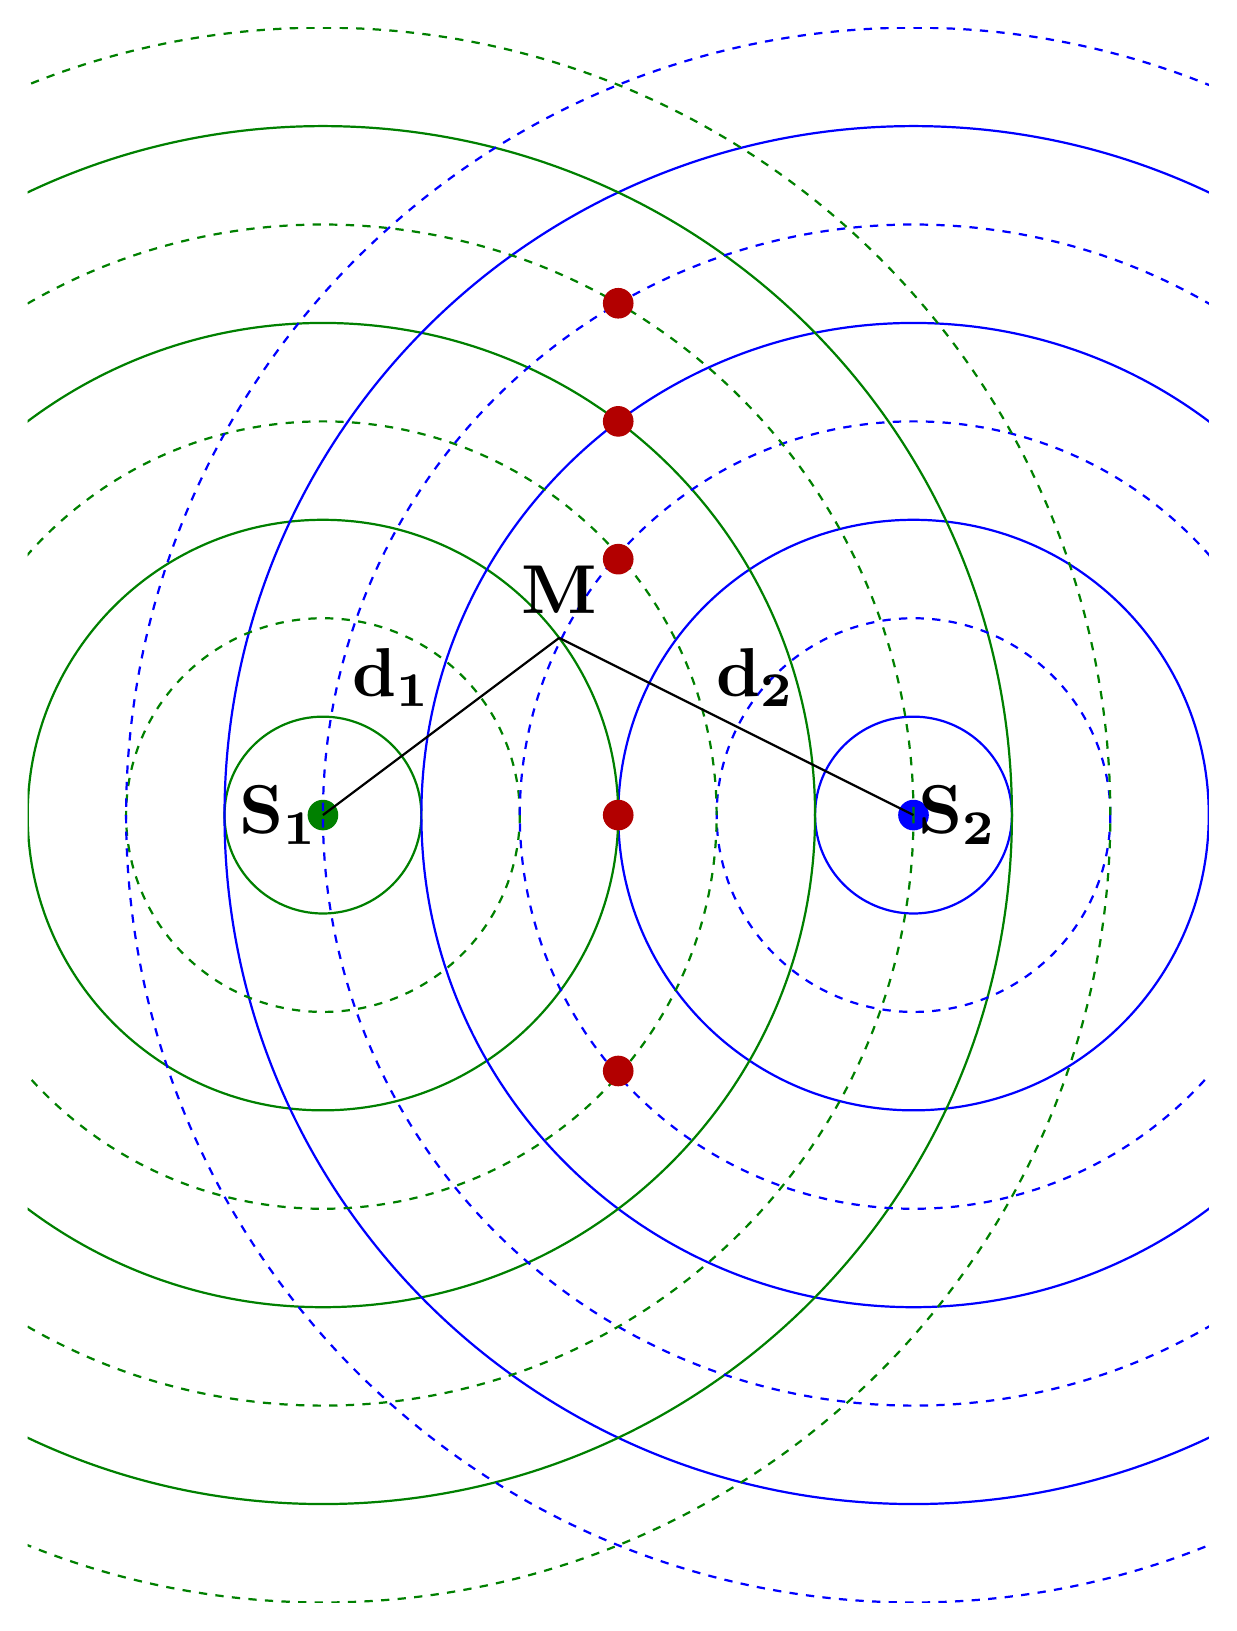
\begin{tikzpicture}[scale=2.5, transform shape]
    \clip(-3,-4) rectangle(3,4);
    \filldraw[blue](1.5,0) circle(.075cm);
    \filldraw[green!50!black](-1.5,0) circle(.075cm);

    \foreach \k in {.5,1.5,2.5,3.5}
      {
        \draw[blue, thick] (1.5,0) circle(\k);
        \draw[green!50!black,thick] (-1.5,0) circle(\k);
      }
    
    \foreach \k in {1,2,3,4}
      {
        \draw[blue, thick, dashed] (1.5,0) circle(\k);
        \draw[green!50!black,thick, dashed] (-1.5,0) circle(\k);
      }

      %% Légendes %%
      \filldraw[red!70!black](0,-1.3) circle(.075cm);
      \filldraw[red!70!black](0,0) circle(.075cm);
      \filldraw[red!70!black](0,1.3) circle(.075cm);
      \filldraw[red!70!black](0,2) circle(.075cm);
      \filldraw[red!70!black](0,2.6) circle(.075cm);


      \filldraw[red!10!blue](.3,-.9) node{$\blacktriangledown$};
      \filldraw[red!10!blue](.3,.9) node{$\blacktriangledown$};
      \filldraw[red!10!blue](.35,1.6) node{$\blacktriangledown$};
      \filldraw[red!10!blue](.45,2.2) node{$\blacktriangledown$};

      \filldraw[orange](.5,0) node{$\blacksquare$};
      \filldraw[orange](.8,1.9) node{$\blacksquare$};
      \filldraw[orange](1,2.45) node{$\blacksquare$};

      \draw(-.3,.9) node[above]{\textbf{M}};
      \draw[thick] (-1.5,0) -- (-.3,.9);
      \draw[thick] (1.5,0) -- (-.3,.9);

      \draw(-1.4,0) node[left]{$\mathbf{S_1}$};
      \draw(1.4,0) node[right]{$\mathbf{S_2}$};
      \draw(-1.15,.7) node{$\mathbf{d_1}$};
      \draw(.7,.7) node{$\mathbf{d_2}$};
  \end{tikzpicture}
  \end{center}
\end{figure}

\noindent\colorbox{red!10}
{\centering
  \begin{minipage}{.98\linewidth}
      \textbf{Questions :}
      \begin{enumerate}
        \item A partir du Document~\ref{doc3} déterminer précisément la longueur d'onde $\lambda$ des ondes produites.
        \item Préciser l'état vibratoire des points circulaires résultant de la superposition des deux ondes.
        \item Pour ces points, exprimer en fonction de $\lambda$ les distances $d_1$ et $d_2$, puis la différence de chemin $\delta = d_1 - d_2$.
        \item Répéter les deux questions précédentes pour les points triangulaires et carrés.
        \item Exprimer les relations liant la différence de chemin $\delta = d_1 - d_2$ et $\lambda$ dans le cas d'interférences constructives et dans le cas d'interférences destructives.
      \end{enumerate}
  \end{minipage}
}
\end{document}